If we compare figur \ref{fig:q25a} and \ref{fig:q25b}, it is clert that
the grafs are very are like, bot \ref{fig:q25a} makes the line betwin
the to classes liner and figur \ref{fig:q25b} maks are more smuts line,
that take som of the destribution i caunt. overall the quadratik
solution is better, bot not by mots.

\begin{figure}[!htbp]
  \centering
  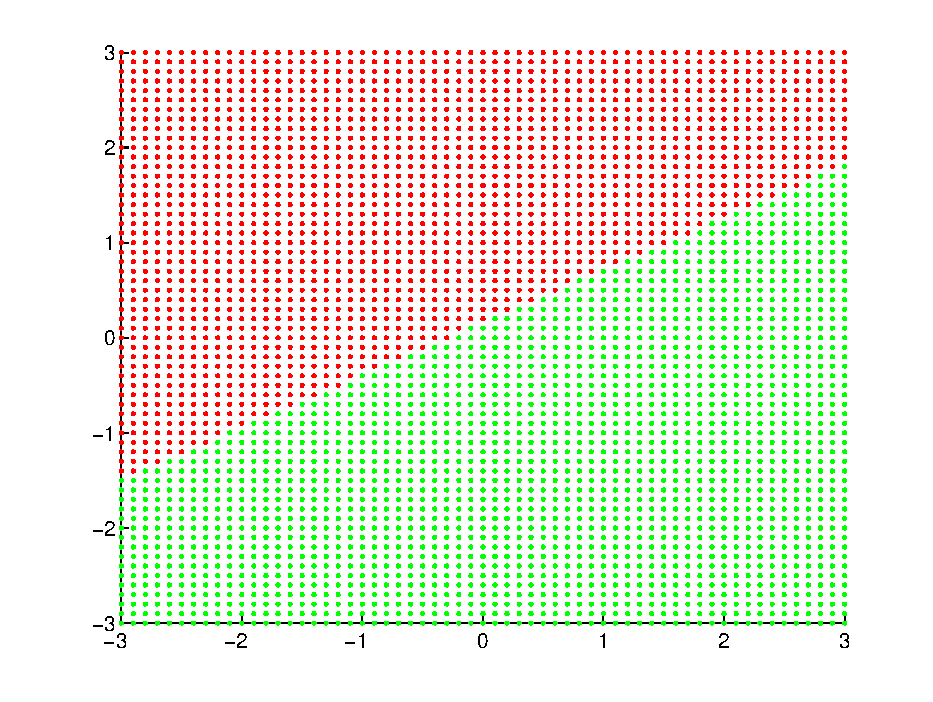
\includegraphics[width=0.6\textwidth]{./images/q25a.pdf}
  \caption{$\phi = (1,x)$, N1 = 250, N1= 250}
  \label{fig:q25a}
\end{figure}

\begin{figure}[!htbp]
  \centering
  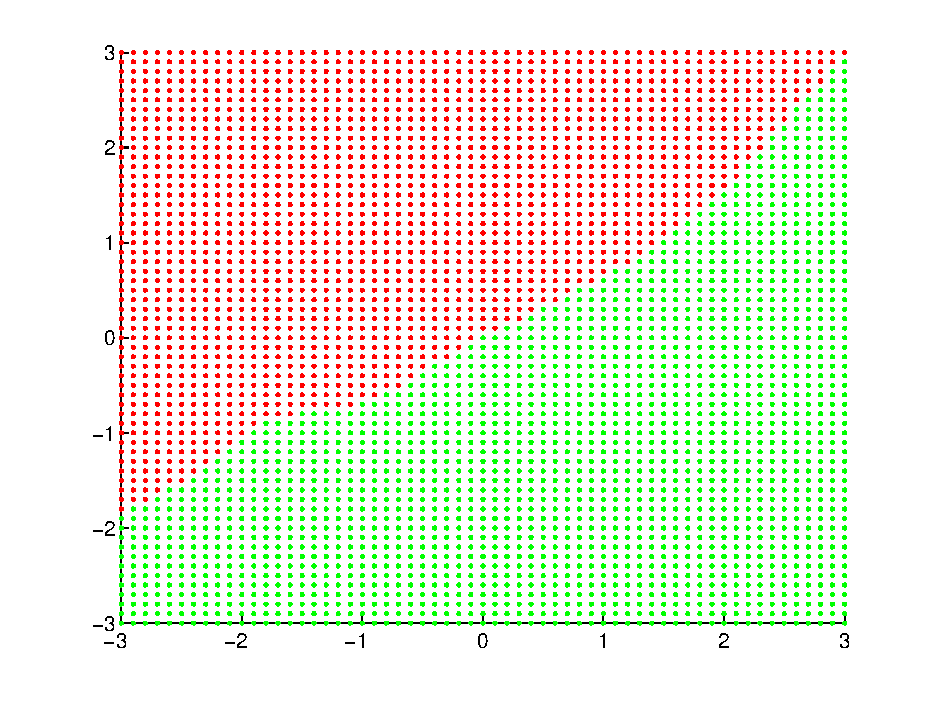
\includegraphics[width=0.6\textwidth]{./images/q25b.pdf}
  \caption{$\phi = (1,x, x^2)$, N1 = 250, N1= 250}
  \label{fig:q25b}
\end{figure}
